\documentclass[11pt,
  titlepage=false,
  %parskip=half,      % enable if you want paragraphs separated by vertical spacing instead of indents
]{scrreprt}

% Style settings
\usepackage[utf8]{inputenc}
\usepackage{microtype}
\usepackage[T1]{fontenc}
\usepackage{lmodern}
\usepackage{siunitx}
\addtokomafont{disposition}{\rmfamily}

\usepackage[bsc,             % for Bachelor's Thesis titlepage
%project,        % for Master's Project titlepage
    claim,iaik]{iaikthesis}

\makeatletter\patchcmd{\scr@startchapter}{\if@openright\cleardoublepage\else\clearpage\fi}{}{}{}\makeatother

% Useful packages for complex content:
\usepackage{amsmath,amsfonts,amssymb} % typesetting math
%\usepackage{siunitx}                 % typesetting SI-units and formatted numbers
%\usepackage{listings}                % typesetting source code
\usepackage{booktabs,multirow}        % utils for complex/beautiful tables
%\usepackage{subcaption}              % placing multiple subfigures in a figure
%\usepackage{graphicx}                % including external image files
%\usepackage{tikz}                    % drawing figures within LaTeX

% Bibliography, referencing, and indexing
\usepackage{csquotes}                 % typesetting \enquote{text in quotes} correctly
\usepackage[backend=biber,
            style=alphabetic,
            minalphanames=3, maxalphanames=4,
            maxbibnames=20]{biblatex} % to generate the bibliography
\addbibresource{report.bib}           % name of the bib-file

% Useful utils:
%\usepackage{todonotes}               % add ToDo markers (\todo{...}, \todo[inline]{...})
\usepackage[hidelinks]{hyperref}
\usepackage{textcomp}
\usepackage{graphicx}
\usepackage{listings}      % clickable links (but hide color frames around links)
%\usepackage{cleveref}                % named references (\Cref{chap:introduction}, ...)

% Your own macros:
%\newcommand{\mynewmacro}[1]{my content with one input parameter: #1}


\usepackage{color}
\definecolor{lightgray}{rgb}{.9,.9,.9}
\definecolor{darkgray}{rgb}{.4,.4,.4}
\definecolor{purple}{rgb}{0.65, 0.12, 0.82}
\lstdefinelanguage{JavaScript}{
  keywords={break, case, catch, continue, debugger, default, delete, do, else, false, finally, for, function, if, in, instanceof, new, null, return, switch, this, throw, true, try, typeof, var, void, while, with},
  morecomment=[l]{//},
  morecomment=[s]{/*}{*/},
  morestring=[b]',
  morestring=[b]",
  ndkeywords={class, export, boolean, throw, implements, import, this},
  keywordstyle=\color{blue}\bfseries,
  ndkeywordstyle=\color{darkgray}\bfseries,
  identifierstyle=\color{black},
  commentstyle=\color{purple}\ttfamily,
  stringstyle=\color{red}\ttfamily,
  sensitive=true
}

\lstset{
   language=JavaScript,
   backgroundcolor=\color{lightgray},
   extendedchars=true,
   basicstyle=\footnotesize\ttfamily,
   showstringspaces=false,
   showspaces=false,
   numbers=left,
   numberstyle=\footnotesize,
   numbersep=9pt,
   tabsize=2,
   breaklines=true,
   showtabs=false,
   captionpos=b
}

\begin{document}

%--- FRONT MATTER --------------------------------------------------------------

%--- INSERT INFORMATION FOR TITLEPAGE ------------------------------------------

% Your name + previous academic degrees:
\thesisauthor{Christoph Royer}

% Title of your thesis:
\thesistitle{JavaSQUIP\\An application of a scheduler queue-based covert channel to JavaScript}

% Date of completion:
\thesisdate{Month Year}

% Supervisor:
%\supervisortitle{Supervisors}
\supervisor{%
    Advisor: Stefan Gast\\
    Supervisor: Daniel Gruss
    \smallskip

    Institute of Applied Information Processing and Communications\\
    Graz University of Technology
}

% Name of your degree programme according to your curriculum
\curriculum{Computer Science}

\printthesistitle

\chapter*{\centering\Large Abstract}
\label{ch:abstract}
The implementation of out-of-order execution has brought a big performance benefit to current CPUs.
But with this benefit also come security concerns, since attackers can exploit the timing variations which are bound to occur in an out-of-order pipeline.
Attacks which target only one execution unit through a separate scheduler queue -- as seen in the Apple M1 and AMD Zen 3 and Zen 4 microarchitectures -- have proven even more powerful than port contention on single-scheduler systems.
As with any attack, porting this side channel to the web would greatly increase its reach and number of victims.

In this thesis, we present the JavaSQUIP attack, which is a port of SQUIP~\cite{squip} to JavaScript.
We look into the security measures used in common browsers to prevent timing attacks, and show how we worked around them successfully.

Our covert channel can provide communication across separate browser instances at a speed of 1000 bits/s,
which is faster than any current covert channel of this type.
At this speed, we were able to achieve a transmission accuracy of $99.2\%$ and $99.3\%$ on Zen 3 and Zen 4 respectively.

Modern CPUs are becoming ever more complex, and with this complexity come more possibilites for side-channel attacks.
JavaSQUIP makes it clear that the security measures of current browsers have not yet adapted to protect against these kinds of attacks.
Our findings suggest that making these attacks impossible may not even be feasible because the drawbacks in performance and features would be too large.
\paragraph{Keywords:}
Covert channel $\cdot$
Scheduler queue contention $\cdot$
JavaScript $\cdot$
AMD Zen

\clearpage

%--- INTRODUCTION --------------------------------------------------------------

\chapter{Introduction}
\label{ch:introduction}

Nowadays, CPU manufacturers are in a steady competition against each other to make their products faster and faster.
One of the ways this is achieved is \textit{out-of-order execution}, where instructions are not executed in program order,
but rather as soon as their respective dependencies are ready and a suitable execution unit is free.
Although this toes the line of breaking the hardware-software contract, the CPU ensures that out-of-order execution remains transparent to the user.
To better balance usage of its execution units, modern CPUs often also include \textit{Simultaneous Multithreading} (SMT).
Here, one physical core is split up into two logical cores, which share physical infrastructure like the schedulers and execution units.

Though out-of-order execution and SMT are designed to be transparent to the user, attacks like
PortSmash~\cite{Aldaya2019port} and SMoTherSpectre~\cite{Bhattacharyya2019} show that the combination of the two forms a viable attack surface.
By measuring timing variations in out-of-order execution, an attacker can gain insight into sensitive information.
This attack, which targets all CPUs with SMT, is called \textit{port contention}.
%Because the instructions are reordered on the fly, the CPUs scheduler needs to distribute incoming instructions across the ports for its several specialized execution units.
If the attacker is co-located with the victim on the same core, they can measure delays when issuing instructions to a shared execution unit.
In this way, the attacker can gain knowledge on the victim's execution based on whether instructions are delayed by the scheduler or not.

SQUIP~\cite{squip} focuses on CPUs with multiple specialized scheduler queues to implement \textit{scheduler queue contention}.
Because each scheduler deals with fewer execution units, the attacker can push one of the comparatively small scheduler queues close to its capacity.
If the victim also adds to the queue, the pipeline stalls, which results in a significant increase in execution time.
This makes SQUIP a fast and reliable covert channel on many modern CPU architectures such as the AMD Zen 3 and Zen 4.~\cite{squip}

Since implementations of port contention-based side channels in a browser setting already exist~\cite{Rokicki2022webport}, we ask the following research question:

\textit{
    Can per-execution-unit scheduler queue contention be exploited in a browser setting?
    Are there significant benefits compared to single scheduler port contention-based approaches?
}

In this thesis, we present JavaSQUIP, a browser-based covert channel based on the SQUIP~\cite{squip} attack.
We show that it is reliable and faster than approaches based on CPU architectures with a single scheduler queue.
We develop a framework for transmitting data between separate instances of a browser at speeds of up to 1000 bit/s.

\paragraph{Outline.}
In Section~\ref{ch:background}, we provide relevant background information on pipelines, schedulers and scheduler queue contention.
We also observe several challenges that we will have to overcome when implementing a timing attack in a browser.
Section~\ref{ch:implementation} shows how we dealt with these challenges and how we optimised JavaSQUIP for speed and reliability.
We go into more detail on the mode and results of our evaluation of JavaSQUIP in Section~\ref{ch:evaluation}.
Section~\ref{ch:conclusion} concludes by comparing JavaSQUIP's performance to similar attacks and outlining potential use cases.
%TODO: reorganise


%--- BACKGROUND ----------------------------------------------------------------

\chapter{Background}
\label{ch:background}

In this chapter, we go into detail on two aspects of CPU scheduling
-- \textit{Out-Of-Order Execution} and \textit{Simultaneous Multithreading} --
and how they have been exploited by prior work.
Furthermore, we take a closer look into the browser features needed to implement these exploits in JavaScript.

\section{Out-Of-Order Execution}
\label{sec:outoforderexecution}
For performance reasons, modern CPUs use efficiency features at almost every stage of an instruction's execution.
One notable feature is \textit{Out-Of-Order Execution},
where instructions are split up into smaller parts.
These so-called \textit{\textmu ops} can be executed in a diffent order than the program order,
enabling a more efficient utilisation of the CPU's resources.

The following paragraphs describe the stages of an instruction in a CISC CPU,
where Out-Of-Order Execution is utilised.

\paragraph{Fetch.}
Before an instruction can be executed, it needs to be loaded from cache or memory.
As branches can make loading unpredictable and loading the wrong instruction is expensive, a \textit{branch prediction unit} tries to guess which path is more likely to be loaded.
Taking this one step further, the predicted path may also be executed before the condition for the branch has been computed.
This is called \textit{speculative execution}\cite{AMD2020OptimizationEPYC7002}.

% TODO: Are there attacks against the decoder too?
\paragraph{Decode.}
Modern CISC CPUs divide normal instructions into their parts when possible;
these parts are called \textit{micro-ops} (\textmu ops)\cite{AMD2020OptimizationEPYC7002}.
For example, an addition with memory operands may be split up into three \textmu ops: one for loading the operands, one for the addition, and one for storing the result.
These \textmu ops can be distributed across specialized execution units, enabling more parallelisation and load balancing, and thus an increase in performance.

\paragraph{Schedule/Execute.}
Once created, the \textmu ops are queued to be executed as soon as their dependencies are met -- sometimes out of the order of their arrival.
Depending on the CPU microarchitecture, there can be one general scheduler queue for all execution units, or multiple.
While Intel uses one scheduler queue for all its execution units~\cite{Intel_opt},
architectures like AMD's Zen~2~\cite{AMD2020OptimizationEPYC7002}, Zen~3~\cite{AMD2020OptimizationEPYC7003} and Zen~4~\cite{AMD2023OptimizationZen4} use several specialized scheduler queues.
When multiple scheduler queues are used, different queues can be specialized for a specific \textmu op or class of \textmu ops.
Figures \ref{fig:amdzen2} and \ref{fig:amdzen3} illustrate the concept.
Splitting the scheduler queue reduces complexity and enables more efficient power usage.

\begin{figure}
    \centering
    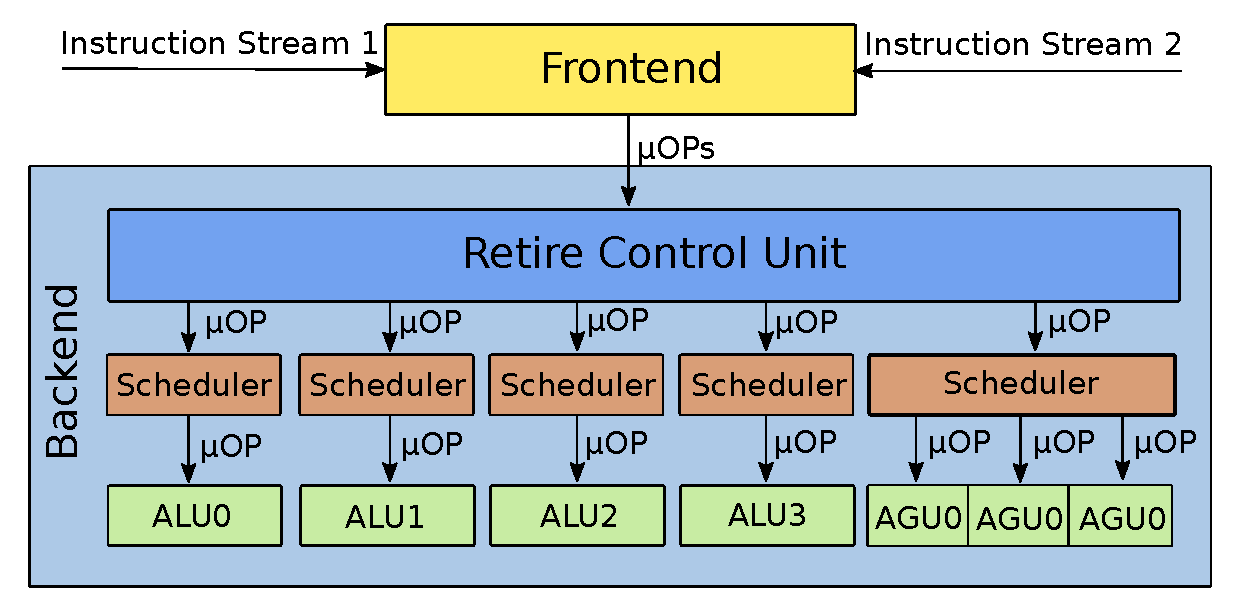
\includegraphics[width=0.5\textwidth]{figures/Zen2 arch}

    \caption{The scheduler layout in AMD Zen~2 (c.f.~\cite{AMD2020OptimizationEPYC7002})}
    \label{fig:amdzen2}

    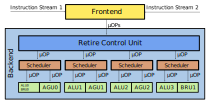
\includegraphics[width=0.5\textwidth]{figures/Zen3 arch}

    \caption{The scheduler layout in AMD Zen~3 (c.f.~\cite{AMD2020OptimizationEPYC7003})}
    \label{fig:amdzen3}
\end{figure}

\paragraph{Retire.}
After all the \textmu ops of an instruction have completed, the \textit{retire control unit} (RCU) reassembles the results.
It commits the finished instructions and schedules dependent instructions -- the dissection into \textmu ops is transparent to the user.

\section{Simultaneous Multithreading}
\label{sec:smt}

As we described in more detail in Chapter~\ref{sec:outoforderexecution},
the cores of a modern CPU are subdivided into multiple specialized execution units.
If only one thread would be executed on such a core,
most of these execution units would stay unused while an instruction is executed.

With \textit{Simultaneous Multithreading} (SMT), one physical core is split into two logical cores~\cite{tullsen1995simultaneous}.
This means that one core executes two threads simultaneously, distributing the workload across its execution units more effectively.
This provides a potential speed-up of up to $100\%$
(realistic tests show a performance gain of about $25\%$~\cite{Phoronix2018HT, Cutress2020SMT})
with relatively little additional architecture needed.

The two threads that are being executed on the same core are called \textit{co-located}.
Usually, these threads should be unaffected by each other; no data is exchanged between two co-located threads.
However, the sharing of common architecture, particularly the execution units,
makes possible several different side-channels -- most of them timing attacks.
A selection of these will be explained in the following chapter.

\section{Exploits}
\label{sec:exploits}
Many of the stages of an instruction's life cycle are exploitable;
in the following, we will list some of the exploits that have already been found.
Each of the attacks outlined in this chapter relies on the attacker being co-located with the victim,
i.e. being executed on the same physical core.

\paragraph{Speculative Execution.}
Executing a path before the condition for the branch is known --
can be exploited, as was shown by Spectre~\cite{spKocherHFGGHHLM019}.

First, the branch prediction unit is primed by repeatedly branching with the condition set to \textit{A}.
In the second step, the branch is called again, but with the condition set to \textit{B}.

Since the branch prediction unit was trained to expect condition \textit{A},
the CPU can be tricked into executing an inaccessible path.
Under the right circumstances, this can be used to leak data from a co-located process.

\paragraph{Port Contention.}
SMoTherSpectre~\cite{Bhattacharyya2019} and PortSmash~\cite{Aldaya2019port} exploit port contention.
They use the fact that only one of the two threads in an SMT-enabled core can use an execution unit in a single cycle.
The attacker can thus find out whether the victim is using a port by measuring the execution time of an instruction on the same port.
Delayed execution gives away the fact that the victim is currently using that port.
Port contention works independently of the type of scheduler queue used.
It affects only one execution unit, and thus creates stalls and measures execution time with the same instruction.

\paragraph{Scheduler Queue Contention.}
SQUIP~\cite{squip} on the other hand exploits scheduler queue contention.
In scheduler queue contention, the attacker fills up the scheduler queue to the point that it is almost at its capacity limit;
any activity of the victim that involves this scheduler queue will overflow the queue, leading to a queue stall.
A queue stall occurs when more \textmu ops of a particular type are created than what the correlating scheduler queue can hold.
Because the CPU cannot drop any \textmu ops, it has to stall the loading of new instructions entirely until the scheduler queue is free again.
The attacker can measure this easily because it entails a significant increase in execution time --
not only for instructions in the affected queue, but on the whole core.
Figure~\ref{fig:amdzen2sqc} shows how one instruction stream can stall the other just by filling up the relatively small scheduler queue.

\begin{figure}
    \centering
    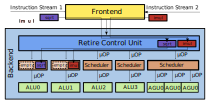
\includegraphics[width=0.75\textwidth]{figures/Zen2 normal operation}

    \caption{An AMD Zen~2 processor in normal operation: the two instruction streams do not impede each other}
    \label{fig:amdzen2normaloperation}

    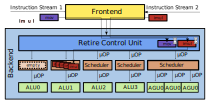
\includegraphics[width=0.75\textwidth]{figures/Zen2 sqc}

    \caption{An AMD Zen~2 processor exhibiting scheduler queue contention: a stall on the Scheduler queue for ALU1 stalls both instruction streams}
    \label{fig:amdzen2sqc}
\end{figure}

SQUIP is limited in its applicable CPU architectures because it relies on the split-scheduler architecture of AMD Zen~2, Zen~3 and Zen~4 CPUs to distinguish between \textmu ops.
However, its advantage is a higher transmission rate compared to port contention.
Because scheduler queue contention stalls the whole CPU, as compared to port contention stalling just one execution unit,
a comparatively bigger increase in execution time is achieved.
Additionally, SQUIP creates very few instuctions on the execution unit where execution times are measured,
since stalls are produced on another unit.
This means that the measured execution unit goes from low load to being stalled completely (see Figure~\ref{fig:amdzen2normaloperation} and Figure~\ref{fig:amdzen2sqc}).
All of this increases the signal-to-noise ratio of the timing measurement,
enabling shorter time slices per bit.
All of this makes SQUIP~\cite{squip} a faster and more reliable side channel than port-contention based side channels.
Because of this advantage, JavaSQUIP aims to port this vulnerability to a browser environment.


\section{Browser security measures}
\label{sec:browsersecurity}
Since the advent of many timing side- and covert channels~\cite{noack2018exploiting, Rokicki2022webport, gruss2016rowhammer, 185126},
browser developers have implemented many measures to mitigate the threat~\cite{shusterman2021prime, performancenow, performancenowchrome, schwarz2018javascript}.
This has always meant striking a balance between security and efficiency.
Because of this, many potential attack surfaces cannot be eliminated without unreasonable losses in performance and functionality,
though some measures do slow down side- and covert channels significantly.

In the following we expand on security measures regarding multithreading, accurate timing in browsers, and low-level operations.
All three of these are needed to mount the SQUIP attack.


\subsection{Timing functions}\label{subsec:timingjs}
There are two contenders for timing measurements in JavaScript: \texttt{Date.now()}~\cite{datenow} and \texttt{performance.now()}~\cite{performancenow}.

The \texttt{Date.now()}~\cite{datenow} function gives a synchronised Unix epoch timestamp with millisecond accuracy.
The Unix epoch time is essentially the time elapsed since January 1, 1970 and is the same for all processes on a computer.
This makes \texttt{Date.now()} a cross-instance synchronised timestamp.

\texttt{performance.now()}~\cite{performancenow} measures the time elapsed since the \textit{time origin} of the current context.
This means that \texttt{performance.now()} gives different values between browser instances, and even between a main thread and its worker threads.
Timing information from \texttt{performance.now()} can still be synchronised;
The \textit{time origin} of the context is given by the \texttt{performance.timeOrigin()}~\cite{performancetimeorigin} property.
This way, the timestamps from \texttt{performance.now()} can be globally synchronised.

The accuracy of \texttt{performance.now()} has been heavily restricted by browsers to counteract the threat of timing attacks.
For example, in Firefox it has an accuracy of 1 ms, and in Chrome it measures with an accuracy of 0.1 ms~\cite{performancenow, performancenowchrome}.

Consequently, both \texttt{Date.now()} and \texttt{performance.now()} give a synchronised timestamp with 1 ms accuracy, making them viable options for synchronisation.

\subsection{Multithreading}\label{subsec:multithreading}
Though JavaScript does not support low-level control over threading, the \texttt{Web Workers} API~\cite{webworkers} allows the user to create workers running in a separate thread.
An instantiated worker runs a predefined script.
The main thread can interface with the worker via calls to the \texttt{Worker.postMessage()} function and via a \texttt{SharedArrayBuffer}~\cite{sharedarraybuffer}.
There is no support for selecting a core on which a worker is run on, presenting a challenge to co-locate with the sender.

Creating a \texttt{SharedArrayBuffer} is restricted in two ways: the browser window needs to be SSL-encrypted, and it needs to restrict some Cross-Origin requests.
Nevertheless, this is not a problem for this attack since the site provides \texttt{https} and all code comes from a single origin.
With the help of free, easy-to-use ssl certificates such as certbot~\cite{certbot}, almost every website on the internet provides an SSL-encrypted connection.
This means that the requirements for a \texttt{SharedArrayBuffer} are likely to be met for any public website a malicious actor would target.

\subsection{Low-level operations in JavaScript}\label{subsec:lowleveljs}
JavaScript handles numbers as floats by default.
This means that a simple invocation of a multiplication like \texttt{a * b;} in JavaScript will not result in an \texttt{imul} instruction on the CPU.
Rather, \texttt{Math.imul(a, b)}~\cite{mathimul} gives the user a lower-level command:
It interprets the parameters as \SI{32}{\bit} integers and multiplies them as such, resulting in an \texttt{imul} instruction on the CPU.
We checked which instructions were generated by running code through V8 -- the compiler used in Chrome --
using the JavaScript explorer on godbolt.org~\cite{godbolt}.

The following function:
\begin{lstlisting}[language=JavaScript]
function test(a) {
    a = Math.sqrt(a);
    a = Math.sqrt(a);
    a = Math.sqrt(a);
    a = Math.sqrt(a);
    a = Math.sqrt(a);
    return a;
}
\end{lstlisting}
contained the following instructions when compiled:
\begin{lstlisting}
0x62a1e00040aa    6a  c5fb104103           vmovsd xmm0,[rcx+0x3]
0x62a1e00040af    6f  c5fb51c0             vsqrtsd xmm0,xmm0,xmm0
0x62a1e00040b3    73  c5fb51c0             vsqrtsd xmm0,xmm0,xmm0
0x62a1e00040b7    77  c5fb51c0             vsqrtsd xmm0,xmm0,xmm0
0x62a1e00040bb    7b  c5fb51c0             vsqrtsd xmm0,xmm0,xmm0
0x62a1e00040bf    7f  c5fb51c0             vsqrtsd xmm0,xmm0,xmm0
0x62a1e00040c3    83  c5fb2cc8             vcvttsd2si rcx,xmm0
0x62a1e00040c7    87  c5832ac9             vcvtlsi2sd xmm1,xmm15,rcx
0x62a1e00040cb    8b  c5f92ec8             vucomisd xmm1,xmm0
\end{lstlisting}

Similarly, \texttt{Math.sqrt()}~\cite{mathsqrt} translates to the \texttt{sqrt} instruction:
\begin{lstlisting}[language=JavaScript]
function test(a) {
    a = Math.imul(a, a);
    a = Math.imul(a, a);
    a = Math.imul(a, a);
    a = Math.imul(a, a);
    a = Math.imul(a, a);
    return a;
}
\end{lstlisting}
\begin{lstlisting}
0x6469d68040b8    78  0f80ba000000         jo 0x6469d6804178  <+0x138>
0x6469d68040be    7e  8bc9                 movl rcx,rcx
0x6469d68040c0    80  8bf9                 movl rdi,rcx
0x6469d68040c2    82  0faff9               imull rdi,rcx
0x6469d68040c5    85  8bcf                 movl rcx,rdi
0x6469d68040c7    87  0fafcf               imull rcx,rdi
0x6469d68040ca    8a  8bf9                 movl rdi,rcx
0x6469d68040cc    8c  0faff9               imull rdi,rcx
0x6469d68040cf    8f  8bcf                 movl rcx,rdi
0x6469d68040d1    91  0fafcf               imull rcx,rdi
0x6469d68040d4    94  8bf9                 movl rdi,rcx
0x6469d68040d6    96  0faff9               imull rdi,rcx
0x6469d68040d9    99  488bcf               REX.W movq rcx,rdi
0x6469d68040dc    9c  03cf                 addl rcx,rdi
0x6469d68040de    9e  0f8046000000         jo 0x6469d680412a  <+0xea>
\end{lstlisting}

%--- IMPLEMENTATION ----------------------------------------------------------------
\chapter{Implementing JavaSQUIP}
\label{ch:implementation}
As described in Section~\ref{sec:browsersecurity}, there are some challenges to overcome when implementing a timing attack in a browser.
This chapter explains how we worked around these challenges to implement the JavaSQUIP covert channel.

\section{General architecture}
We built a showcase for JavaSQUIP consisting of two web pages: one receiver and one sender.
The aim was to build a showcase that, while showing the capabilities of the covert channel,
should reflect as realistic a scenario as possible to also prove the feasibility of a side channel attack.
The difference between a side channel and a covert channel is that a side channel attack involves a (non-cooperating) victim and
an attacker, while covert channels have a cooperating pair of sender and receiver.

The sender in the showcase corresponds to the victim in a side-channel scenario.
Since a victim does not cooperate in an attack, the sender was kept as simple as possible.
It consists of one thread, sending one bit per timeslice (see \ref{sec:accurate-timing}) via issuing \texttt{Math.imul()} instructions or not.

The receiver represents the attacker.
The assumption was that an attacker can execute arbitrary scripts, for example as an interactive advertisement on a website.
Given this, the attacker can get one thread co-located with the victim and exploit the SQUIP sidechannel to gain information.
Details on the implementation are described in the following chapters.

\section{Getting accurate timing}
\label{sec:accurate-timing}
JavaSQUIP needs two kinds of timing in order to work properly:
\begin{itemize}
    \item a cross-process syncronized clock to determine the start of bit transmissions:\\
    resolution of ${f_{\text{transmission}}}^{-1} \approx$ 1ms
    \item a fine-grained measurement to measure port contention:\\
    resolution of 100 CPU cycles $\approx$ 25ns
\end{itemize}

For the synchronised clock, we can use \texttt{Date.now()}~\cite{datenow}, which has a 1ms accuracy.
This allows us to partition the duration of the transmission into 1ms \textit{timeslices}.
During one timeslice, a single bit can be transmitted by the existence or absence of port contention.
The alignment of bytes is solved by starting the transmission on a multiple of 8 timeslices since the start of the epoch (see \ref{subsec:timingjs}).
Synchronising with \texttt{Date.now()}~\cite{datenow} works, but only for transmissions of up to 1000 bits/s,
since there is no more precise timestamp in JavaScript which is synchronised across browser instances.

%To get around this and realize a faster transmission than 1000 bits/s, we propose implementing the Manchester Code~\cite{manchesterEncoding}.
%It is self-synchronising, which eliminates the need for an external source of synchronisation.
%The actual implementation is not within the scope of this thesis.

The receiver also needs a way to measure the small variations in timing whenever a scheduler queue gets blocked.
Since no timing function in JavaScript gives a better accuracy than 0.1ms, we need to provide our own timing.

We solved this with a counting worker, which continually increases one variable in the \texttt{SharedArrayBuffer}.
As explained in section \ref{subsec:multithreading}, the other receiver workers can then access this counter and use it to measure execution times with adequate accuracy.
The paper on \textit{Fantastic Timers}~\cite{Schwarz2017Timers} does an excellent job on explaining the concept in-depth.

\section{Co-locating with the sender}
\label{sec:co-location}
For co-locating the receiver with the sender, the receiver creates as many receiving workers as the number of virtual cores in the machine, minus two:
one for the counting thread (see \ref{sec:accurate-timing}), and one for the sending thread.
In our experiments, we used an \textit{AMD Ryzen 7 5800X} as representative for Zen~3 and an \textit{AMD Ryzen 7 7700X} as representative for Zen~4.
Both are 8-core CPUs, so the experiments were run with $8 \times 2 - 2 = 14$ receiver workers.
Since every thread does continuous work, each thread will most likely be assigned to a unique virtual core.

To receive the message, one of the worker threads needs to be co-located with the sending thread.
Assuming a uniform distribution for the threads, we can calculate the theoretical co-location probability.
The only way that the sender is not co-located with a receiver is that the sender is co-located with the counting thread,
which is a $\frac{1}{15}$ chance.
Thus, the theoretical co-location probability is $\frac{14}{15} \approx 93.3\%$

To figure out which receiver is the one co-located with the sender,
we need to take advantage of some characteristic of the transmission.
With some optimisations of the receiver workers -- described closer in \ref{sec:reducecontention} --
we were able to get the contention of two co-located receiver workers very low.
The counting thread does not cause much contention either.
This means that if a \texttt{1} is sent, the sender will cause the highest scheduler queue contention level -- i.e. the longest execution time --
among all the physical cores.
Detecting the correct receiver worker is now a matter of selecting the receiver with the highest contention;
this will correctly identify the co-located receiver if a \texttt{1} is sent, and a random receiver if a \texttt{0} is sent.
Since in this case all receivers report low contention, a \texttt{0} is still registered regardless of the selected receiver.

% TODO: better graphic, with axes and stuff
\begin{figure}
    \centering
    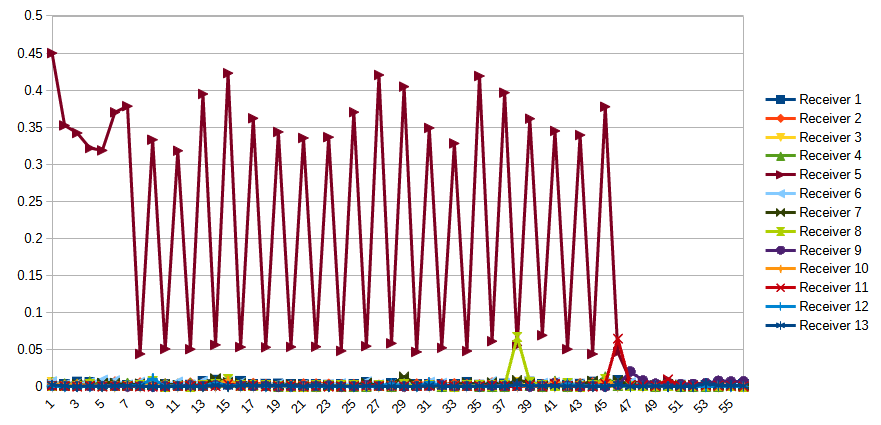
\includegraphics[width=0.75\textwidth]{figures/contentiontest}

    \caption{Execution time per timeslice during a test run of sending alternating \texttt{0}'s and \texttt{1}'s}
    \label{fig:contentiontest}
\end{figure}

Figure~\ref{fig:contentiontest} displays the contention of each receiver for each timeslice.
One can easily see that receiver 5 is co-located with the sender;
it registers alternating high and low contention, in accordance with the alternating \texttt{1}'s and \texttt{0}'s sent by the sender.
Meanwhile, the contention measured by the other receivers stays low.

\section{Targeting a scheduler queue}
JavaSQUIP targets AMD Zen~2, Zen~3 and Zen~4;
these architectures support multiplication only on ALU1~\cite{AMD2020OptimizationEPYC7003}.
When sending a 1, JavaSQUIP makes multiple codependent calls to \texttt{Math.imul()}, which translate to the \texttt{imul} instruction.
This fills up the scheduler queue of ALU1, eventually causing a queue stall.
The codependence of the \texttt{imul} operations ensures that they have to be executed one after the other, in order.
It is ensured simply by using the result of one operation as the input for the next.

The following code snippet shows two functions of the sending process.
The functions are for sending a zero or a one respectively, in a given time frame.
The parameter \texttt{until} gives the end of the timeslice to send a bit.
\begin{lstlisting}[language=JavaScript]
function send_zero(until) {
  until = +until;

  while(+Date.now() < +until) {
    // simply busy waiting
  }
}

function send_one(until) {
  until = +until;

  let i = dummy[0]|0;
  let j = dummy[1]|0;
  while(+Date.now() < until) {
    i = (((i|0) + 100069) % 100103) | 0;
    j = (((j|0) + 997) % 13) | 0;

    // block scheduler queue with 100 imul instructions
    i = Math.imul(i|0, j|0) | 0;
    i = Math.imul(i|0, j|0) | 0;
    // repeats 100 times
    i = Math.imul(i|0, j|0) | 0;
    i = Math.imul(i|0, j|0) | 0;
  }

  // use the result so the calculation is not optimised away
  dummy[1] ^= i|0;
}
\end{lstlisting}

\section{Detecting scheduler queue contention}
\label{sec:detect-sqc}
The receiving process needs to detect whether the sender has sent a \texttt{1} or a \texttt{0}.
This is equivalent to detecting scheduler queue contention.
This was implemented by issuing several \texttt{imul} instructions,
and measuring the delay with the help of a separate counting thread.

The following code snippet shows how the receiver issues 10 \texttt{sqrt} and 20 \texttt{imul} instructions,
retreiving the counter value before and after.
If the retire control unit was not blocked by an overflowing scheduler queue,
the instructions can be reordered so both reads of the counting value are right after one another.
This results in the measured time delay being zero, which means no scheduler queue contention took place.
If the two values are not equal, we can deduce that scheduler queue contention is in progress.
% TODO reads weird

\begin{lstlisting}[language=JavaScript]
function squip(start_value, factor) {
  start_value = +start_value;
  factor = factor|0;

  let dummy = +start_value;

  let start_time = Atomics.load(timer, 0)|0;

  dummy = +Math.sqrt(+dummy);
  dummy = +Math.sqrt(+dummy);
  // repeats 10 times
  dummy = +Math.sqrt(+dummy);
  dummy = +Math.sqrt(+dummy);

  dummy = dummy|0;

  dummy = Math.imul(dummy|0, factor|0)|0;
  dummy = Math.imul(dummy|0, factor|0)|0;
  // repeats 20 times
  dummy = Math.imul(dummy|0, factor|0)|0;
  dummy = Math.imul(dummy|0, factor|0)|0;

  let end_time = Atomics.load(timer, 0)|0;

  return {
    dummy: dummy|0,
    time: ((end_time|0) != (start_time|0))|0
  };
}
\end{lstlisting}

The \texttt{squip} function is run repeatedly, summing up the return values of each iteration.
At the end of the timeslice, this sum is compared to a threshold.
If it is above the threshold, a \texttt{1} is registered, else a \texttt{0}.

\section{Optimisation}
JavaSQUIP is intended to show SQUIP's potential as an attack in a browser setting.
Because of this, we aimed to make it as fast and stable as possible.

\subsection{Delay threshold}
The simplest parameter in SQUIP is the delay threshold.
It determines whether the summed up delay of a timeslice is registered as a \texttt{0} or a \texttt{1}.
If the threshold is too high or too low, results are skewed towards registering a \texttt{0} or a \texttt{1} respectively.

To tune this parameter, the resulting bitstream was checked against the actual sent stream.
All of the bits that were wrongly registered as \texttt{1} or wrongly \texttt{0} were tallied up separately.
Then the delay threshold was adjusted until faulty \texttt{1}'s and faulty \texttt{0}'s were approximately equally frequent,
meaning that no skew toward high or low bits is present and the delay threshold is set optimally.

Figure~\ref{fig:contentiontest} shows the contention of every reciever thread during such a test.
It shows that a threshold value of $0.2$ would be optimal, giving the best margin for \texttt{0}- and \texttt{1}-transmissions.


\subsection{Number of instructions for a queue stall}
The sender blocks a targeted scheduler queue by sending a large number of instructions to it.
The number of instructions is another tunable parameter:
it needs to be big enough to cause a queue stall and a spike in execution time,
yet it needs to be as small as possible to minimise chance of a stall bleeding into the following timeslice.

To tune the number of \texttt{imul} instructions, a bleed-over test was constructed.
It test consists of a string of alternating \texttt{1}s and \texttt{0}s, so contrasts between different bits could be easily observed.
The amount of \texttt{imul} instructions was tuned by successively reducing the number and running a test.
% TODO how many did you have in the end?
As soon as no spike in execution time was registered, the lower limit was found.
Figure~\ref{fig:contentiontest} shows the final tuned system;
the spikes for a \texttt{1} are pronounced, while the execution time in a \texttt{0}-timeslice is only slightly higher than for the remaining receivers.

\subsection{Minimising contention by the receivers}
\label{sec:reducecontention}
% todo a single one? und homma nid wos ondas gmessn?
The receiver detects a queue stall by measuring the time delay for an \texttt{imul} instruction.
To get a more stable result, several successive \texttt{imul} instructions were used.
The goal here was to get reliable results, while minimising the contention caused by the receivers themselves.
This is helpful in the transmission, as it reduces the contention for two co-located receivers,
maximizing the contrast to the receiver that is co-located with the sender (see \ref{sec:co-location})

The detection test was constructed similarly to the bleed-over test:
alternating \texttt{1}s and \texttt{0}s were received, and the delays measured.
The number of \texttt{imul} instructions in the receiver worker was reduced until no signal was retreivable,
resulting in a lower bound for the number of \texttt{imul} instructions in the receiver worker.
% todo what is the lower bound you found, as a number?

In addition to tuning the number of \texttt{imul} instructions, two more optimisations were done in the receiver worker:
buffer instructions and a delay loop.

In the measurement function, 10 \texttt{sqrt} instructions serve as a buffer to delay the \texttt{imul} instrucions:
they delay the execution, while not creating contention on ALU1.
% todo hmmm they delay the multiplications, hence they also extend the period of time where there is contention.
The implementation can be seen in section~\ref{sec:detect-sqc}.

A delay loop was added after each measurement to give the scheduler queue time to recover from the interference of the measurement.
% todo not clear what was meant here
Since no normal delay function gives a better accuracy than 1ms, a busy-waiting loop was used.
The following code shows the delay loop that was executed after each measurement.
\begin{lstlisting}[language=JavaScript]
let k = 0|0;
while(k < 1000|0) {
  dummy  ^= k|0;
  k += 1;
}
\end{lstlisting}

Figure~\ref{fig:contentiontest} demonstrates these measures working:
Receiver 5 -- which is co-located with the sender -- receives a clean signal of alternating \texttt{1}'s and \texttt{0}'s.
Meanwhile, all the remaining receivers -- which are co-located either with each other or with the counting thread -- show very little contention.

\pagebreak
%--- EVALUATING JAVASQUIP --------------------------------------------------------------
\chapter{Evaluating JavaSQUIP}
\label{ch:evaluation}

% todo different approaches not clear - explain better
To evaluate and measure different approaches, we set up a test scenario for JavaSQUIP.
It consists of two web pages communicating with each other solely over JavaSQUIP.

\section {Test setup}
\label{sec:testsetup}
Our aim was to evaluate JavaSQUIP on both the Zen~3 and Zen~4 architecture.
To this end, we tested on an \textit{AMD Ryzen 7 5800X} as representative for Zen~3 and an \textit{AMD Ryzen 7 7700X} as representative for Zen~4.

The test setup constists of two webpages: a sender and a receiver.
The sender simulates the target, and the receiver simulates a page that is controlled by the attacker.
Because the attacker has little or no control over the target, we kept the sender page minimal.
The sender has only one working thread.
The working thread is sending either a 0 (no action) or a 1 (contention with codependent \texttt{Math.imul()} calls) for each timeslice.
With more control over the receiver, the attacker can ensure co-location from this side.
For our tests on the \textit{AMD Ryzen 7 5800X}(Zen~3) and \textit{AMD Ryzen 7 7700X}(Zen~4), we needed 14 receiving workers.
We go into more detail on co-location in Chapter~\ref{sec:co-location}.

To distinguish a message from random noise on the CPU, the sender sends a preamble before the actual data.
The preamble is a sequence of the numbers from 100 through 109.
If the receiver sees two ascending bytes between 100 and 109, it is highly likely that this is part of the preamble --
a message was detected.
For easier evaluation of the transmission accuracy, the message is also stored on the receiver's side,
so that the number of "faulty \texttt{1}" and "faulty \texttt{0}" bits can be automatically calculated.
In our test setup, messages of 500 random bytes were sent at a transmission speed of 1000bits/s.
This results in a transmission time of $\frac{500 \times 8}{1000} = 4$ seconds.

\section{Speed}
The sender and receiver need to know the desired transmission speed beforehand to match up their timeslices.
This means that the transmission speed is a fixed value and needs no further calculation.
Due to the reduced resolution of the Date.now() timer used for the time slices (see Section~\ref{sec:accurate-timing}),
our best achievable speed was 1000bits/s.

There is, however, still some overhead for the preamble (see Section~\ref{sec:testsetup}).
It is a fixed size of 10 bytes regardless of the message,
so the relative overhead tends to $0\%$ as the message size increases.

\section{Reliability}
There are two aspects that affect the reliability of the covert channel:
First, the sender being co-located with a receiver, and second, the resilience of the covert channel against noise.

To measure the actual co-location probability, we used the preamble system as described in Section~\ref{sec:testsetup}.
Threads are unlikely to be relocated during the 4 seconds of a transmission,
and the preamble is likely to be recognised if co-location is given (see noise resilience further down).
We can conclude that the rate of recognised preambles is a good measurement for the actual co-location probability.
Further, the resilience to noise can be measured by the accuracy of a message when the preamble was recognised.

In our tests, we found an average co-location probability of $88.7\%$ in a Zen~3 architecture and $96\%$ in Zen~4.
This is consistent with the theoretical $93.3\%$ calculated in Section~\ref{sec:co-location}.
When tested under stress with \texttt{stress --cpu 1}, we achieved an average co-location probability of $53.7\%$.

For measuring noise resistance, we only looked at those transmissions where the preamble was recognised.
This resulted in an average transmission accuracy of $99.2\%$ on Zen~3, and $99.3\%$ on Zen~4.
With \texttt{stress --cpu 1}, we observed an accuracy of $74\%$.

\ref{fig:contentiontest_stress} shows the effect of outside CPU stress on the measurement.
Although the \texttt{stress} command creates more noise in the measurement, the overall contention levels go down (compare with \ref{fig:contentiontest}).
This is because \texttt{stress} does not target a specific scheduler queue, but instead takes up CPU time with a varied set of instructions.
The result is more relocation of threads (the sending thread is first co-located with receiver 13, later with receiver 7), and less contention.

\begin{figure}
    \centering
    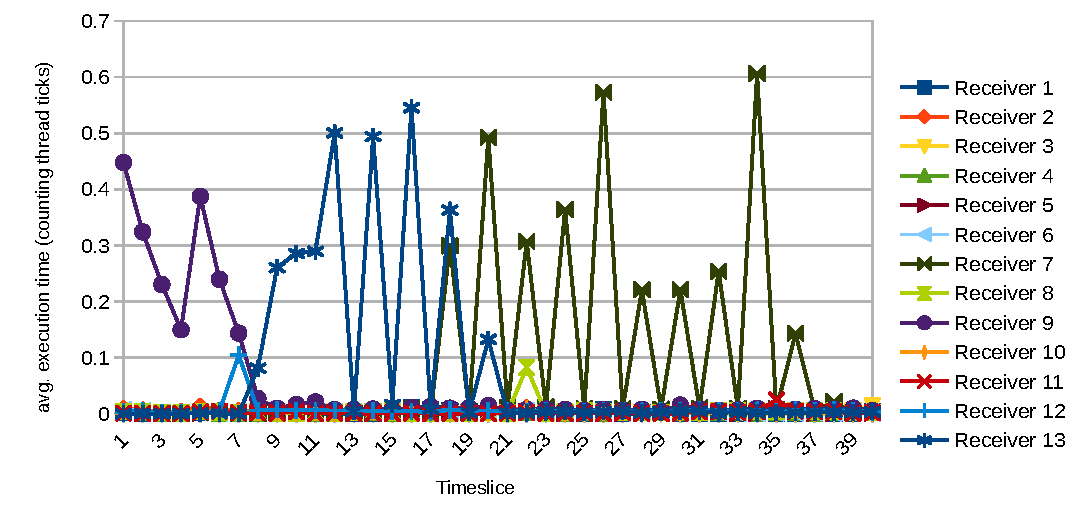
\includegraphics[width=0.75\textwidth]{figures/contentiontest_stress}

    \caption{Execution time per timeslice during a test run of sending alternating \texttt{0}'s and \texttt{1}'s with \texttt{stress --cpu 1}}
    \label{fig:contentiontest_stress}
\end{figure}

%--- CONCLUSION ----------------------------------------------------------------

\chapter{Conclusion}
\label{ch:conclusion}
In this thesis, we ported the SQUIP~\cite{squip} attack to a JavaScript context, thus creating the JavaSQUIP covert channel.
JavaSQUIP has achieved a transmission rate of 1000 bits/s, proving an advantage in performance over attacking single-scheduler based architectures~\cite{Rokicki2022webport}.
Additionally, we proved a co-location rate of $88.7\%$/$96\%$ with a transmission accuracy of $99.2\%$/$99.3\%$ (Zen~3/Zen~4).
This shows that architectures with multiple scheduler queues present a bigger attack surface than their single-scheduler counterparts.

JavaSQUIP breaks the sandboxing model of a web browser context.
This means that one browser instance can communicate with another without using the network, thus being virtually undetectable for an unknowing victim.
This could potentially be used by malicious code within a website -- no matter its origin -- to exfiltrate data to another browser instance on the same computer.
Its speed and accuracy enable an attacker to transmit large amounts of data, such as images or short audio clips, within the lifetime of a malicious web page.

Though security updates in modern browsers slow down and hinder timing attacks, microarchitectural attacks have not yet been eliminated.
JavaSQUIP mostly uses JavaScript features that have already been restricted to improve security as much as feasible;
mitigating microarchitectural attacks in a browser setting proves to be increasingly hard as CPUs grow more and more complex.


%--- BIBLIOGRAPHY --------------------------------------------------------------
\pagebreak
\printbibliography

\end{document}
